\chapter{Conception du système}

\rhead{Conception du système}
\lfoot{\leftmark}

\section{Introduction}
Ce chapitre présente la conception de la plateforme de triage automatique des incidents Apache Spark. Après avoir étudié les choix technologiques dans le chapitre précédent, nous nous concentrons ici sur l'organisation concrète du système. Nous commençons par une analyse approfondie du jeu de données exploité, en décrivant sa structure, ses volumes et ses spécificités. Nous présentons ensuite la modélisation du processus de traitement à travers l'architecture en médaillon mise en œuvre avec dbt et Snowflake. Enfin, nous décrivons l'architecture générale du système, en détaillant les composants d'intelligence artificielle qui constituent le cœur de la plateforme : le pipeline de classification hybride fondé sur les embeddings de transformers, le mécanisme de routage par confiance et l'arbitrage par modèle de langage.

%--------------------------2-----------------------------
\section{Analyse et description du jeu de données}

\subsection{Origine et nature des données}

Il convient de souligner que la plateforme développée dans le cadre de ce stage est déployée en environnement de production au sein de SQLI, où elle traite des données réelles issues des tickets d'un client de l'entreprise. Cependant, des obligations contractuelles de confidentialité interdisent la divulgation de ces données ainsi que la présentation de résultats obtenus à partir de celles-ci dans un document académique. Afin de permettre la validation scientifique de l'approche et d'assurer la reproductibilité des résultats présentés dans ce rapport, un jeu de données public de nature et de structure équivalentes a été retenu comme support de démonstration. Il s'agit d'un export du gestionnaire de tickets JIRA de la fondation Apache, mis à disposition sur la plateforme Kaggle en mars 2025. Cet export couvre l'ensemble des projets hébergés par la fondation Apache, représentant un volume brut d'environ 8,7 gigaoctets de données tabulaires au format CSV. Conformément au périmètre du projet, seuls les tickets associés au projet Apache Spark ont été retenus, soit environ 49 832 tickets sur un total de plus d'un million d'entrées dans le fichier d'issues. Ce filtrage est appliqué dès la première couche de transformation par la condition \texttt{project\_key = 'SPARK'}.

Les données sont réparties en quatre fichiers sources distincts, chacun représentant une entité du système JIRA. Ces fichiers entretiennent des relations entre eux via les identifiants de tickets, permettant de reconstituer le cycle de vie complet d'un incident, depuis sa création jusqu'à sa résolution.

\subsection{Description des fichiers sources}

Le tableau \ref{tab:dataset} présente les quatre fichiers sources composant le jeu de données, avec leurs volumes respectifs et les informations qu'ils contiennent.

\begin{table}[h!]
\centering
\begin{tabularx}{\textwidth}{|c|c|X|}
  \hline
  \textbf{Fichier} & \textbf{Nombre de lignes} & \textbf{Contenu principal} \\
  \hline
  issues.csv & 1 149 321 & Tickets de tous les projets Apache : résumé, description, type d'incident, résolution, priorité, statut, reporter, assignataire, dates de création et de mise à jour \\
  \hline
  comments.csv & 5 047 714 & Commentaires associés aux tickets : auteur, corps du commentaire, horodatage \\
  \hline
  changelog.csv & 9 653 526 & Journal des modifications de chaque ticket : champ modifié, valeur avant, valeur après, auteur, date de la modification \\
  \hline
  issuelinks.csv & 390 063 & Relations inter-tickets : type de lien (blocks, duplicates, relates to, etc.), ticket source, ticket cible \\
  \hline
\end{tabularx}
\caption{Description des fichiers sources du jeu de données}
\label{tab:dataset}
\end{table}

\subsection{Structure et caractéristiques des tickets}

Chaque ticket Apache Spark est décrit par un ensemble de champs structurés et semi-structurés. Les champs structurés comprennent l'identifiant unique du ticket (clé JIRA de la forme SPARK-XXXXX), le type d'incident (\textit{issuetype}), la résolution (\textit{resolution}), la priorité (\textit{priority}), le statut courant (\textit{status}), ainsi que les informations relatives aux utilisateurs impliqués (reporter et assignataire).

Les champs textuels constituent la principale source d'information sémantique. Le résumé (\textit{summary}) offre une description synthétique en une ligne, tandis que la description (\textit{description}) peut contenir plusieurs paragraphes incluant des extraits de code, des traces d'exécution (stack traces), des liens vers des ressources externes et des balises HTML issues de l'interface JIRA. Ces particularités imposent un traitement NLP spécifique avant toute exploitation par le pipeline de classification.

\subsection{Normalisation des étiquettes de classification}

L'objectif du pipeline est de prédire deux cibles pour chaque nouveau ticket : le type d'incident (\textit{issuetype}) et la résolution probable (\textit{resolution}). Or, dans les données brutes, ces champs présentent une hétérogénéité importante due à des valeurs saisies librement par les contributeurs au fil des années.

Pour le type d'incident, on dénombre 22 valeurs brutes distinctes, dont certaines sont redondantes ou marginales. Une table de correspondance (\textit{issuetype\_mapping.csv}), intégrée comme \textit{seed} dbt, les regroupe en 9 classes normalisées couvrant les catégories principales : Bug, Improvement, New Feature, Task, Sub-task, Test, Wish, Question et Documentation.

Pour la résolution, 15 valeurs brutes sont normalisées en 7 classes via la table \textit{resolution\_mapping.csv} : Fixed, Won't Fix, Duplicate, Cannot Reproduce, Not A Problem, Later et Incomplete.

\subsection{Découpage temporel et volume final}

Afin de garantir une évaluation rigoureuse du pipeline de classification, les données Apache Spark sont partitionnées selon l'axe temporel de création du ticket. Ce découpage évite toute contamination entre les ensembles d'entraînement et d'évaluation, les tickets les plus récents étant inconnus lors de l'apprentissage. Le tableau \ref{tab:split} détaille la répartition des tickets entre les trois ensembles.

\begin{table}[h!]
\centering
\begin{tabularx}{\textwidth}{|c|X|X|}
  \hline
  \textbf{Ensemble} & \textbf{Période de création} & \textbf{Rôle} \\
  \hline
  Entraînement & Avant 2022 & Base de référence pour la recherche par similarité vectorielle \\
  \hline
  Validation & Année 2022 & Calibration des hyperparamètres (k, seuils de confiance, poids des boosts) \\
  \hline
  Test & Année 2023 & Évaluation finale, utilisé une seule fois après verrouillage des paramètres \\
  \hline
  Exclu & Données incomplètes ou ambiguës & Non utilisé dans le pipeline \\
  \hline
\end{tabularx}
\caption{Découpage temporel du jeu de données Apache Spark}
\label{tab:split}
\end{table}

Après application de l'ensemble des règles de filtrage et de nettoyage, le volume final traité dans la table intermédiaire \textit{INT\_ISSUES\_CLEANED} s'élève à 45 043 tickets, auxquels sont associés 41 986 enregistrements de commentaires agrégés, 29 937 entrées de caractéristiques issues du journal de modifications et 11 179 enregistrements de caractéristiques de liens inter-tickets.

%--------------------------3-----------------------------
\section{Modélisation du processus de traitement}

\subsection{Vue d'ensemble : architecture en médaillon}

Le processus de traitement des données est structuré selon l'architecture en médaillon, organisée en trois couches de qualité croissante au sein de la base de données Snowflake \textit{PFE\_SPARK}. Chaque couche correspond à un niveau de maturité de la donnée, depuis l'ingestion brute jusqu'aux tables de consommation finales. L'ensemble des transformations est orchestré par dbt, qui gère les dépendances entre les modèles sous forme de graphe acyclique dirigé (DAG) et garantit l'exécution des tests automatisés à chaque étape. La figure \ref{fig:medallion_flow} illustre l'enchaînement des couches et les schémas Snowflake correspondants.

\begin{figure}[H]
    \centering
    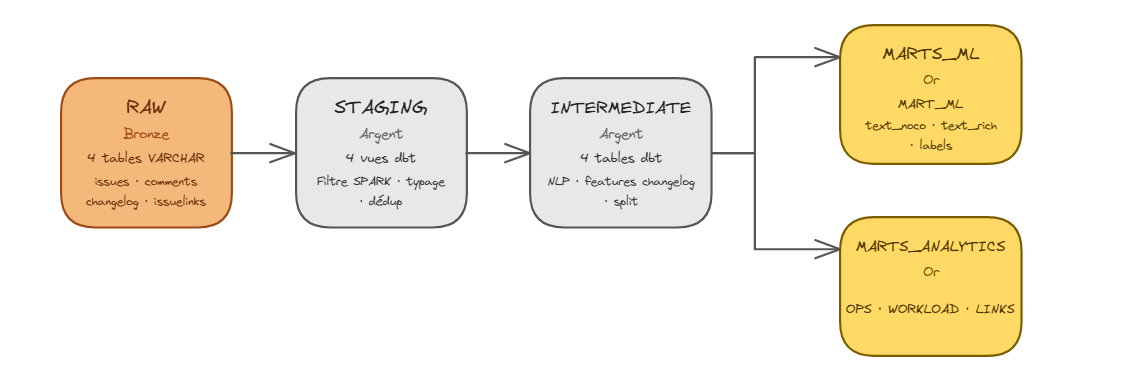
\includegraphics[width=\textwidth]{images/medallion_flow.png}
    \caption{Architecture en médaillon du processus de traitement}
    \label{fig:medallion_flow}
\end{figure}

\subsection{Couche Bronze : ingestion brute}

La couche Bronze constitue le point d'entrée des données dans la plateforme. Les quatre fichiers CSV sources sont chargés dans Snowflake en deux étapes. La commande \texttt{PUT} transfère les fichiers compressés depuis le système de fichiers local vers le stage interne Snowflake. La commande \texttt{COPY INTO} exécute ensuite l'ingestion vers les tables cibles. Toutes les colonnes sont stockées au format \texttt{VARCHAR}, reproduisant fidèlement la structure CSV d'origine grâce à un mapping positionnel (\texttt{\$N}). Aucune transformation métier n'est appliquée à ce stade, préservant ainsi un historique immuable qui permet de retraiter les couches supérieures à tout moment sans dépendre de la source originale.

\subsection{Couche Argent — Staging : filtrage mécanique}

La couche Staging est implémentée sous forme de vues dbt directement au-dessus des tables Bronze. Son rôle est de réaliser un ensemble d'opérations mécaniques de préparation : filtrage des tickets au seul projet Apache Spark, renommage des colonnes selon les conventions du projet, transtypage vers les types natifs Snowflake (entiers, dates, booléens) et déduplication. Pour le journal de modifications, un filtre supplémentaire est appliqué afin de ne retenir que les changements portant sur les champs métier pertinents : statut, priorité, résolution, assignataire et type d'incident. Ce filtrage réduit le volume du changelog de 9,6 millions à environ 400 000 entrées exploitables.

\subsection{Couche Argent — Intermédiaire : logique métier et ingénierie des caractéristiques}

La couche Intermédiaire porte l'essentiel de la valeur ajoutée du processus de traitement. Elle est implémentée sous forme de tables dbt matérialisées, calculées à partir des vues de Staging.

\subsubsection{Nettoyage textuel et normalisation des étiquettes}

Le modèle \textit{INT\_ISSUES\_CLEANED} applique une macro dbt de nettoyage NLP en six étapes successives sur les champs textuels : suppression des balises HTML, retrait des blocs de code délimités par des backticks, élimination des mentions d'utilisateurs (format @username), suppression des URLs, normalisation des espaces multiples, et mise en minuscule. En parallèle, les étiquettes brutes de type et de résolution sont remplacées par leurs valeurs normalisées via les seeds dbt \textit{issuetype\_mapping} et \textit{resolution\_mapping}. Enfin, une colonne \textit{split} est calculée pour chaque ticket selon sa date de création, affectant la valeur \textit{train} (avant 2022), \textit{val} (2022) ou \textit{test} (2023).

\subsubsection{Agrégation des commentaires}

Le modèle \textit{INT\_COMMENTS\_AGGREGATED} consolide les commentaires de chaque ticket selon la politique « premiers 5 + derniers 3 ». Cette heuristique capture à la fois le contexte initial de signalement, généralement exprimé dans les premiers échanges, et les éléments de résolution, qui apparaissent naturellement en fin de fil de discussion. Le texte agrégé résultant est intégré dans la vue enrichie du ticket (\textit{text\_rich}), qui constitue la seconde entrée du pipeline d'embedding.

\subsubsection{Extraction des caractéristiques du journal de modifications}

Le modèle \textit{INT\_CHANGELOG\_FEATURES} extrait des indicateurs comportementaux à partir du journal des modifications. L'indicateur \textit{was\_escalated} détecte si la priorité d'un ticket a été revue à la hausse au cours de son cycle de vie. Son calcul repose sur un mapping des étiquettes de priorité vers des entiers ordonnés (Blocker~=~4, Critical~=~3, Major~=~2, Minor~=~1, Trivial~=~0), permettant une comparaison numérique correcte que la comparaison alphabétique des chaînes de caractères ne permettrait pas. L'indicateur complémentaire \textit{was\_deescalated} capte le phénomène de baisse de priorité. L'indicateur \textit{n\_assignee\_changes} comptabilise le nombre de réassignations successives, signal révélateur de la complexité ou de l'ambiguïté du ticket. Ces caractéristiques sont utilisées comme signal de reranking dans le pipeline de classification.

\subsubsection{Caractéristiques des liens inter-tickets}

Le modèle \textit{INT\_ISSUELINKS\_FEATURES} calcule pour chaque ticket le nombre total de liens entrants et sortants ainsi que la distribution par type de lien (blocks, duplicates, relates to). Ces métriques fournissent une mesure de la connectivité du ticket dans le graphe des incidents, un signal complémentaire aux informations textuelles.

\subsection{Couche Or : tables de consommation}

La couche Or produit les tables finales destinées à la consommation par le pipeline de classification et par les applications de restitution.

\subsubsection{Mart Machine Learning}

La table \textit{MART\_ML}, hébergée dans le schéma \textit{MARTS\_ML}, constitue le contrat d'interface entre la couche de transformation et le pipeline Python. Elle consolide, pour chaque ticket, deux représentations textuelles complémentaires :

\begin{itemize}
    \item \textbf{text\_noco} : vue minimale du ticket composée du résumé, de la priorité, du statut et du reporter, sans aucune information pouvant agir comme indice sur l'étiquette cible. Cette représentation est conçue pour capturer l'essence du problème signalé.
    \item \textbf{text\_rich} : vue enrichie intégrant les commentaires agrégés et les métadonnées structurées (nombre de commentaires, nombre de liens, indicateurs de changelog). Cette représentation vise à capturer le contexte de résolution.
\end{itemize}

La table inclut également les étiquettes normalisées (\textit{issuetype\_norm}, \textit{resolution\_norm}), la colonne \textit{split} pour le découpage train/validation/test, et les caractéristiques numériques de changelog.

\subsubsection{Marts Analytiques}

Trois tables sont produites dans le schéma \textit{MARTS\_ANALYTICS} pour alimenter le tableau de bord :

\begin{itemize}
    \item \textbf{MART\_ANALYTICS\_OPS} : agrégats mensuels par type d'incident, couvrant l'ensemble des années disponibles sans restriction au seul ensemble d'entraînement.
    \item \textbf{MART\_ANALYTICS\_WORKLOAD} : métriques de charge par assignataire (volume de tickets assignés, délai médian de résolution, taux de clôture).
    \item \textbf{MART\_ANALYTICS\_LINKS} : métriques de connectivité par ticket (degré de liens entrants et sortants, présence de liens de blocage).
\end{itemize}

\subsection{Garanties de qualité}

L'ensemble du pipeline de transformation est couvert par une suite de plus de 50 tests dbt automatisés, répartis sur toutes les couches. Ces tests vérifient l'unicité des clés primaires, l'absence de valeurs nulles sur les colonnes critiques, la conformité des étiquettes normalisées aux valeurs attendues (incluant la valeur "Won't Fix"), et des contraintes de plage pour les indicateurs numériques. L'exécution de la commande \texttt{dbt test} produit un résultat sans aucun avertissement ni erreur, garantissant l'intégrité de la donnée à chaque étape du processus.

%--------------------------4-----------------------------
\section{Architecture générale du système}

\subsection{Vue d'ensemble}

La plateforme se décompose en quatre blocs fonctionnels qui s'articulent de manière séquentielle : la couche d'ingestion, la couche de transformation décrite dans la section précédente, le pipeline de classification hybride fondé sur l'intelligence artificielle, et la couche de restitution. La figure \ref{fig:archi_generale} illustre les flux de données entre ces composants et positionne chaque brique technologique dans l'architecture globale.

\begin{figure}[H]
    \centering
    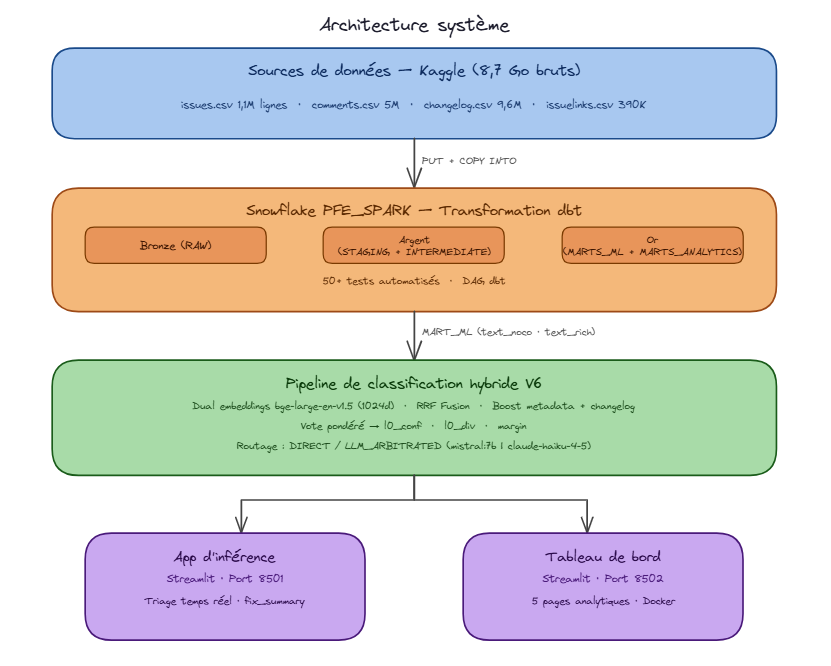
\includegraphics[width=\textwidth]{images/architecture_generale.png}
    \caption{Architecture générale de la plateforme de triage automatique}
    \label{fig:archi_generale}
\end{figure}

\subsection{Composants d'intelligence artificielle : vue d'ensemble}

L'intelligence artificielle intervient à plusieurs niveaux dans la plateforme, tous opérés exclusivement via \textbf{Snowflake Cortex} depuis des requêtes SQL. Cette intégration native garantit que les données ne quittent jamais l'environnement sécurisé Snowflake, ce qui est déterminant dans un contexte de conformité et de gouvernance des données.

Quatre fonctions Cortex sont mobilisées de manière combinée tout au long du pipeline :

\begin{itemize}
    \item \texttt{SNOWFLAKE.CORTEX.COMPLETE('mistral-large2', ...)} pour la summarization technique et l'extraction de mots clés, en raison de son excellent rapport performances/coût sur les tâches de génération structurée en anglais technique.
    \item \texttt{SNOWFLAKE.CORTEX.EMBED\_TEXT\_768('snowflake-arctic-embed-m', ...)} pour le calcul des vecteurs denses de 768 dimensions, natif à Snowflake et optimisé pour la recherche sémantique.
    \item \texttt{VECTOR\_COSINE\_SIMILARITY()} pour la recherche des tickets historiques les plus similaires, directement en SQL, sans bibliothèque externe ni infrastructure dédiée.
    \item \texttt{SNOWFLAKE.CORTEX.COMPLETE('llama3.3-70b', ...)} pour la classification finale par raisonnement few-shot et la génération des résumés correctifs, en raison de sa supériorité sur les prompts complexes avec chain-of-thought.
\end{itemize}

\subsection{Pipeline de classification RAG sur Snowflake Cortex}

Le pipeline de classification constitue le cœur intelligent du système. Il s'articule en cinq étapes séquentielles entièrement implémentées en SQL sur Snowflake, selon une architecture RAG (Retrieval-Augmented Generation) adaptée au contexte du triage de tickets. La figure \ref{fig:rag_archi} illustre le flux global du pipeline.

\begin{figure}[H]
    \centering
    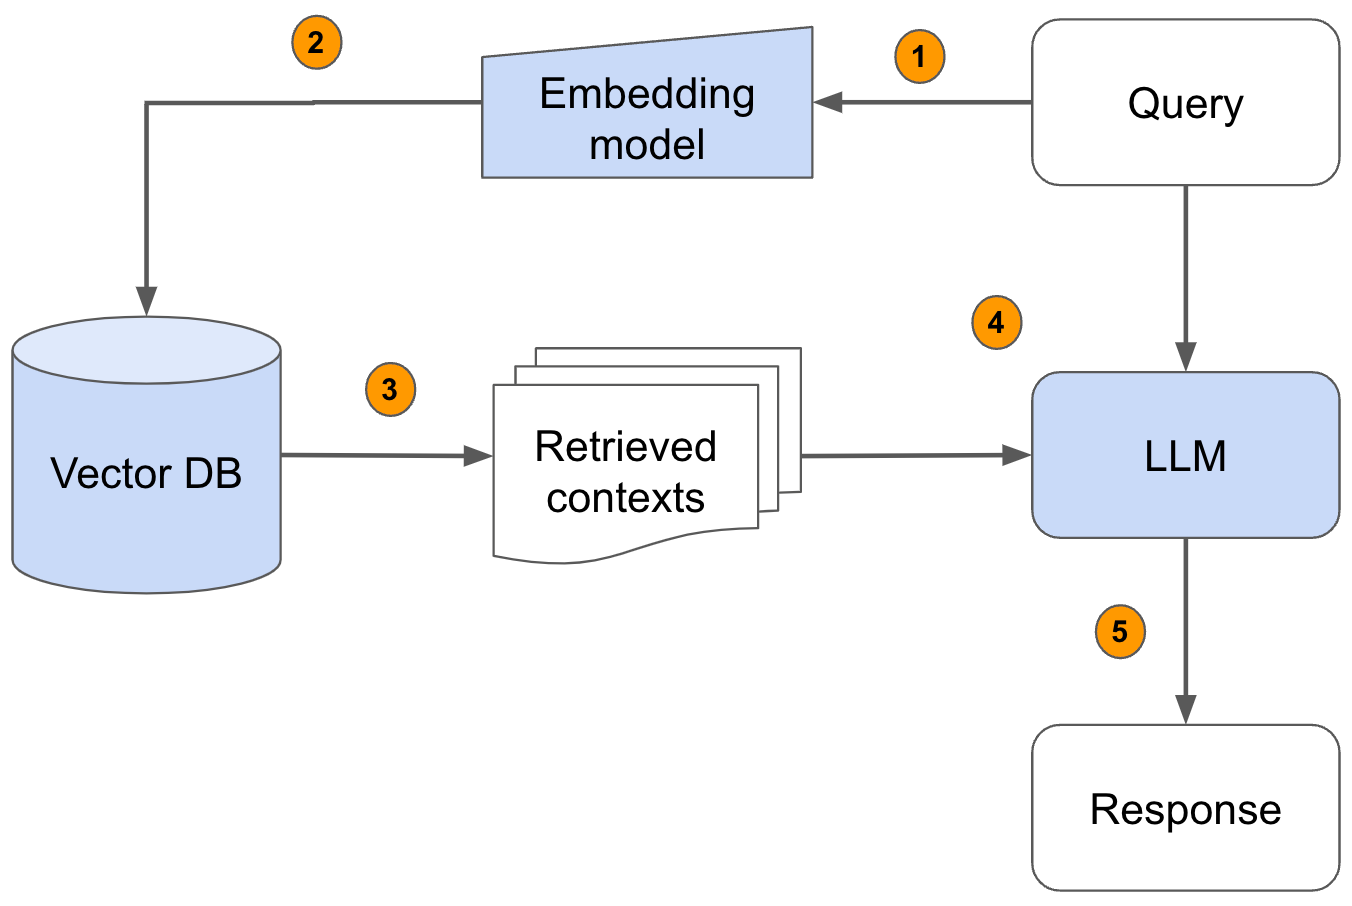
\includegraphics[width=0.85\textwidth]{images/rag_archi.png}
    \caption{Pipeline RAG de classification sur Snowflake Cortex}
    \label{fig:rag_archi}
\end{figure}

\subsubsection{Étape 1 — Construction du texte technique enrichi}

La première étape consiste à construire, pour chaque ticket de la base d'entraînement, une représentation textuelle unifiée à partir des sources disponibles. Les modèles dbt de la couche intermédiaire ont déjà produit les colonnes \textit{text\_noco} et \textit{text\_rich}. Ces représentations sont consolidées dans deux colonnes complémentaires utilisées par les étapes suivantes :

\begin{itemize}
    \item \textbf{INFORMATION\_ONE} : concaténation du résumé nettoyé, de la description et des commentaires agrégés (politique premiers-5 + derniers-3). Cette colonne sert de base pour le calcul des embeddings et les règles de correspondance lexicale.
    \item \textbf{INFORMATION\_TWO} : version étendue intégrant les métadonnées structurées (priorité, statut, indicateurs de changelog). Cette colonne est injectée dans le contexte du prompt LLM final pour enrichir le raisonnement du modèle.
\end{itemize}

Le recours aux commentaires est motivé par leur richesse informationnelle : les premiers commentaires exposent le contexte de signalement du problème, tandis que les derniers contiennent généralement les éléments menant à la résolution, deux signaux complémentaires pour la prédiction du type d'incident et de la résolution probable.

\subsubsection{Étape 2 — Summarization technique et embedding 768 dimensions}

La deuxième étape transforme chaque ticket en une représentation vectorielle dense via un processus en deux temps.

\paragraph{Summarization technique par LLM}

Avant de calculer l'embedding, une étape de summarization est appliquée via \texttt{CORTEX.COMPLETE('mistral-large2', ...)}. Un prompt personnalisé demande au modèle de supprimer tout le bruit du texte brut (balises HTML, URLs, références de tickets, adresses email) et de produire un résumé technique de 3 à 5 phrases ne conservant que le contenu discriminant : le composant défaillant, le système concerné et le comportement observé.

Cette étape est préférée à la fonction native \texttt{CORTEX.SUMMARIZE()} car cette dernière est généraliste et conserve les éléments de bruit. Le prompt personnalisé produit un texte standardisé, plus propre pour l'embedding et comparable entre tickets de styles rédactionnels très différents.

\paragraph{Calcul des embeddings 768D}

Le résumé nettoyé est ensuite encodé par le modèle \texttt{snowflake-arctic-embed-m} via la fonction \texttt{CORTEX.EMBED\_TEXT\_768()}, produisant un vecteur de 768 dimensions stocké nativement dans une colonne de type \texttt{VECTOR(FLOAT, 768)} :

\begin{lstlisting}[language=SQL]
SNOWFLAKE.CORTEX.EMBED_TEXT_768(
    'snowflake-arctic-embed-m',
    COALESCE(SUMMARIZED_ONE, LEFT(INFORMATION_ONE, 512))
) AS EMBEDDING_ONE
\end{lstlisting}

Le \texttt{COALESCE} protège contre les cas où la summarization échoue, en utilisant directement les 512 premiers caractères du texte brut. Les embeddings calculés constituent la base vectorielle de référence du système RAG.

Le choix du modèle \texttt{snowflake-arctic-embed-m} est justifié par trois facteurs convergents : son intégration native dans Snowflake sans aucun transfert de données, ses 768 dimensions offrant un bon équilibre entre précision sémantique et coût de stockage, et ses performances de premier plan sur les tâches de recherche sémantique en anglais technique.

\subsubsection{Étape 3 — Extraction de mots clés techniques}

La troisième étape enrichit chaque ticket d'un ensemble de mots clés techniques extraits par LLM. Un prompt \texttt{mistral-large2} demande au modèle d'extraire les dix termes les plus discriminants du texte du ticket, en se concentrant sur les noms de technologies, de composants, de types d'erreurs et de systèmes impliqués. Ces mots clés sont ensuite agrégés par catégorie cible (\textit{issuetype\_norm}) pour construire un dictionnaire de signatures textuelles : les termes les plus fréquents dans les tickets d'une catégorie constituent son empreinte lexicale distinctive.

La motivation de cette étape est de corriger un biais structurel de la similarité cosinus : deux tickets peuvent être sémantiquement proches sans partager les mêmes termes techniques discriminants. Un ticket mentionnant un \textit{NullPointerException dans le planificateur de tâches} et un ticket évoquant une \textit{exception dans le gestionnaire de ressources} peuvent avoir une forte similarité vectorielle mais relever de catégories différentes. Les mots clés apportent un signal lexical complémentaire au signal sémantique.

\subsubsection{Étape 4 — Recherche par similarité et re-ranking hybride}

La quatrième étape constitue le cœur du pipeline RAG. Pour chaque ticket de validation, le système recherche les tickets d'entraînement les plus similaires, puis re-ranke les résultats par un score hybride combinant similarité sémantique et correspondance de mots clés.

\paragraph{Recherche par similarité cosinus}

Le ticket de validation est d'abord encodé par le même modèle d'embedding que les tickets d'entraînement, garantissant la cohérence de l'espace vectoriel. Il est ensuite comparé à l'ensemble de la base d'entraînement via \texttt{VECTOR\_COSINE\_SIMILARITY()} en SQL. Pour deux vecteurs $\mathbf{a}$ et $\mathbf{b}$ de dimension 768, la similarité cosinus est définie par :

$$\text{sim}(\mathbf{a}, \mathbf{b}) = \frac{\mathbf{a} \cdot \mathbf{b}}{\|\mathbf{a}\| \cdot \|\mathbf{b}\|}$$

Cette métrique est insensible à la norme des vecteurs et mesure uniquement l'alignement directionnel dans l'espace sémantique, ce qui la rend particulièrement robuste aux variations de longueur des textes. Les cinq tickets d'entraînement présentant le score de similarité cosinus le plus élevé sont retenus comme candidats initiaux.

\paragraph{Re-ranking hybride sémantique + mots clés}

Le classement initial est ensuite affiné par un score combiné :

$$\text{COMBINED\_SCORE} = (\text{SIMILARITY\_SCORE} \times 0{,}6) + (\text{keyword\_match\_count} \times 0{,}08)$$

Le \textit{keyword\_match\_count} comptabilise le nombre de mots clés caractéristiques de la catégorie candidate présents dans le texte du ticket à classifier. Ce re-ranking peut inverser le classement initial : un ticket candidat avec une similarité cosinus légèrement inférieure mais partageant davantage de termes techniques discriminants avec la requête remonte dans le classement final.

\subsubsection{Étape 5 — Classification par LLM avec few-shot dynamique}

La cinquième étape soumet les résultats du re-ranking à \texttt{llama3.3-70b} pour produire la prédiction finale. Le modèle \texttt{llama3.3-70b} est retenu pour sa supériorité sur les prompts complexes avec chain-of-thought par rapport à \texttt{mistral-large2}, et pour sa meilleure capacité à suivre des instructions détaillées portant sur plusieurs catégories avec des règles de désambiguïsation explicites.

Un prompt structuré en cinq couches est construit dynamiquement pour chaque ticket :

\begin{enumerate}
    \item \textbf{Définitions des catégories} : toutes les valeurs valides de \textit{issuetype\_norm} et \textit{resolution\_norm} avec leur description, permettant au modèle de comprendre les nuances entre catégories voisines (ex : Bug vs Improvement lorsque le ticket propose un correctif).
    \item \textbf{Règles de désambiguïsation} : construites par analyse des erreurs sur le jeu de validation, ces règles encodent les confusions fréquentes observées empiriquement.
    \item \textbf{Few-shot dynamique re-ranké} : les cinq exemples issus du re-ranking, présentés avec leurs scores de similarité et de correspondance de mots clés, ainsi que leurs étiquettes cibles connues.
    \item \textbf{Catégories candidates restreintes} : seules les catégories effectivement représentées dans le top-5 sont soumises au choix du modèle, réduisant l'espace de décision et améliorant la précision.
    \item \textbf{Chain-of-thought} : une instruction explicite demande au modèle de raisonner en plusieurs étapes avant de formuler sa réponse finale.
\end{enumerate}

La réponse du modèle est ensuite validée syntaxiquement : si la valeur retournée ne correspond pas exactement à l'une des catégories valides, un mécanisme de normalisation par correspondance partielle (\texttt{ILIKE}) la corrige vers la catégorie la plus proche, garantissant que la sortie finale est toujours une étiquette reconnue.

\subsection{Génération des résumés correctifs}

Pour chaque ticket classifié, le pipeline génère un résumé correctif de 1 à 2 phrases décrivant l'analyse de la cause probable de l'incident. Ce résumé est généré par \texttt{llama3.3-70b} dans une requête séparée, \textit{après} que la classification est définitivement fixée. Cette séquentialité est délibérée : générer le résumé dans la même requête que la classification créerait un biais circulaire où le modèle pourrait être influencé par le résumé qu'il est en train de produire, au détriment de la fiabilité de l'étiquette prédite.

Le prompt de génération reçoit le type d'incident prédit, le texte du ticket, le domaine applicatif et la priorité. Il est instruit de commencer par \textit{«~L'incident a été causé par...~»} et de mentionner le composant ou le module spécifique impliqué. La concision maximale (1-2 phrases) garantit des résumés directement exploitables par les équipes de développement, sans nécessiter de reformulation.

\subsection{Couche de restitution}

La plateforme expose deux applications Streamlit pour la restitution des résultats aux utilisateurs finaux.

\subsubsection{Application de triage en temps réel}

L'application d'inférence, accessible sur le port 8501, permet le triage en temps réel d'un nouveau ticket. L'utilisateur saisit le résumé et la description du ticket. L'application appelle le pipeline Cortex SQL, puis affiche la prédiction du type d'incident, la résolution probable et le résumé correctif. Un panneau dédié présente les tickets historiques les plus similaires avec leurs scores de similarité et de correspondance de mots clés, offrant aux développeurs un point de départ concret pour la résolution du problème signalé.

\subsubsection{Tableau de bord analytique}

L'application analytique, accessible sur le port 8502, est une application multi-pages permettant l'exploration des données opérationnelles historiques. Elle est structurée en cinq pages complémentaires alimentées par les tables \textit{MART\_ANALYTICS\_OPS}, \textit{MART\_ANALYTICS\_WORKLOAD} et \textit{MART\_ANALYTICS\_LINKS} :

\begin{itemize}
    \item \textbf{Page 1 — Vue d'ensemble} : évolution mensuelle du volume de tickets et répartition par type d'incident.
    \item \textbf{Page 2 — Résolution} : analyse des délais de résolution et distribution des motifs de clôture.
    \item \textbf{Page 3 — Charge de travail} : tableau de bord par assignataire (volume, délai médian, taux de clôture).
    \item \textbf{Page 4 — Relations} : exploration des liens entre tickets et identification des composants les plus bloquants.
    \item \textbf{Page 5 — Anomalies} : détection de tickets présentant des patterns de changelog anormaux (forte rotation d'assignataires, escalades de priorité, délais de résolution atypiques).
\end{itemize}

%--------------------------5-----------------------------
\section{Conclusion}

Ce chapitre a posé les fondations de la conception de la plateforme de triage automatique. Nous avons présenté le jeu de données Apache JIRA dans sa structure, son volume et ses spécificités, avant de décrire en détail le processus de transformation qui, à travers l'architecture en médaillon pilotée par dbt, produit des tables de consommation fiables et validées par plus de 50 tests automatisés. Nous avons ensuite décrit l'architecture générale du système et détaillé le pipeline RAG implémenté entièrement sur Snowflake Cortex : summarization par \texttt{mistral-large2}, embedding 768 dimensions par \texttt{snowflake-arctic-embed-m}, re-ranking hybride sémantique et mots clés, classification few-shot par \texttt{llama3.3-70b} avec chain-of-thought, et génération de résumés correctifs. Le chapitre suivant sera consacré à la réalisation et à la mise en œuvre de cette architecture, en présentant les aspects d'implémentation et les résultats obtenus sur l'ensemble de test.
